\section{Universality Classes and Critical Scaling under Dropout}

Dropout \cite{srivastava2014dropout,wager2013dropout} is often used as a regularizer that reduces overfitting by randomly masking activations during training, thereby reducing the network's reliance on any single subset of pathways and discouraging co-adaptation. In the previous literature, dropout was explored in MFT \cite{lee2019mean, schoenholz2017deepinformationpropagation}, but not in the universality class sense. We formalize dropout as multiplicative Bernoulli noise applied post-activation,
\begin{equation}
p^{(\ell)}_{j} \sim \mathrm{Bernoulli}(\rho), \qquad y^{(\ell)}_j \;\mapsto\; \tilde y^{(\ell)}_j \equiv \frac{p^{(\ell)}_{j}}{\rho} y^{(\ell)}_j,
\end{equation}
i.e.\ the standard inverted-dropout convention in which $\mathbb E_p[\tilde y^{(\ell)}_j]=y^{(\ell)}_j$, and hence $\mathbb E_p[\tilde z^{\ell+1}_i\mid W,b,y^\ell]=z^{\ell+1}_i$, so the mean preactivation is invariant to the dropout rate \cite{schoenholz2017deepinformationpropagation}. Throughout, $\rho$ is the keep probability. When comparing two inputs, we draw the dropout masks independently for each input\footnote{Correlated dropout masks can alleviate this detuning: if the same mask is shared across the batch, the \(c=1\) fixed point is preserved and near-critical scaling can be recovered by retuning, but the noise becomes batch coupled and the regularization is correspondingly weaker and more structured. We leave detailed analysis of correlated masks to future work.}; this independence is the source of the decorrelation effect analyzed below.

The smooth/kinked distinction also appears in the Hermite expansion of the activation: $\tanh$ has rapidly decaying coefficients, while \relu{} has a power-law tail. These coefficients determine which derivatives of the correlation map remain finite near perfect alignment, connecting activation regularity to the dropout scaling laws (App.~\ref{sec:var-opt-act}).

Our classification is orthogonal to the scale-invariant vs. non-scale-invariant distinction of \cite{roberts2022principlesdeeplearningtheory}: the multi-scale Hermite spectrum highlighted above is controlled primarily by analytic structure, not by scale invariance per se. The criterion is based on two facts: (a) near-critical scaling laws differ between smooth and kinked activations, and (b) ordinary kinks produce power-law Hermite tails, whereas the smooth examples considered here have much faster decay (Apps.~\ref{ap:exponent_derivations} and~\ref{sec:var-opt-act}).

Consider sending exactly the same input through the same network twice. Without dropout, the two representations remain identical at every layer. With independently sampled dropout masks, different coordinates are erased on the two passes, so even identical inputs no longer produce perfectly aligned representations. Rescaling the surviving activations preserves their mean, but does not restore the missing agreement between the two passes. Perfect alignment therefore ceases to be a fixed point, cutting off the divergence of the depth correlation length at the edge \cite{schoenholz2017deepinformationpropagation}. For a single input, the corresponding variance increase can instead be absorbed into an effective weight variance, $\sigma_w^2\mapsto\sigma_w^2/\rho$.

Introducing multiplicative Bernoulli noise with keep probability $\rho$, the perturbed preactivations read
\begin{equation}
z_i^\ell = \frac{1}{\rho} \sum_{j=1}^{N_{\ell-1}} W_{ij}^\ell p_j^{\ell-1} y_j^{\ell-1} + b_i^\ell.
\end{equation}
The single-input variance recursion becomes
\begin{equation}
\bar{q}_{aa}^{\ell} = \frac{\sigma_{w}^{2}}{\rho} \int Dz \phi^{2}\left( \sqrt{\bar{q}_{aa}^{\ell-1}} z \right) + \sigma_{b}^{2},
\end{equation}
where the bar reminds us that the variance fixed point is shifted by dropout. We denote the (putative) dropout variance fixed point by
\begin{equation}
\bar q^{*} \;=\; \frac{\sigma_w^2}{\rho}\int Dz \phi^2\big(\sqrt{\bar q^{*}} z\big) + \sigma_b^2.
\label{eq:qstar-dropout}
\end{equation}
Assuming this variance fixed point exists and is positive, two distinct inputs $a\neq b$ acquire a dropout shift at perfect alignment. If at some depth $c^{\ell}_{ab}=1$, then at the next layer one finds \cite{schoenholz2017deepinformationpropagation}
\begin{equation}
\bar F_\rho(1)= \bar c^{\ell+1}_{ab} = 1 - \frac{1 - \rho}{\rho \bar{q}^{*}} \sigma_{w}^{2} \int Dz \phi^{2}\left( \sqrt{\bar{q}^{*}} z \right).
\end{equation}
It is therefore natural to define the dropout field
\begin{align}
h &\;\equiv\; 1-\bar F_\rho(1)\nonumber\\
&\;=\; \frac{1-\rho}{\rho \bar q^{*}}\; \sigma_w^2\int Dz \phi^2\big(\sqrt{\bar q^{*}} z\big).
\label{eq:Delta_exact}
\end{align}
For a nondegenerate channel with $\sigma_w^2\int Dz\,\phi(\sqrt{\bar q^*}z)^2>0$, construction gives $\rho<1\Rightarrow h>0$,
so the fixed point at $c^*=1$ is immediately spoiled: even if two inputs are perfectly aligned at some depth, the next layer produces $\bar c_{ab}=1-h<1$. Since we focus on weak dropout, it is useful to perform the small-\(\delta\rho\) expansion. Writing $\delta\rho\equiv 1-\rho$ with $\delta\rho\ll 1$, suppose the no-dropout variance fixed point is positive, isolated and stable, with variance-map derivative $|\chi_q|<1$. The implicit-function theorem then gives $\bar q^*=q^*+\mathcal O(\delta\rho)$, so to leading order
\begin{equation}
h = \delta\rho\; \frac{\sigma_w^2}{\bar q^{*}}\int Dz \phi^2\big(\sqrt{\bar q^{*}} z\big) + \mathcal O(\delta\rho^2).
\label{eq:Delta_weakdrop}
\end{equation}
This variance expansion excludes a marginal variance fixed point. For bias-free \relu{} at unchanged He initialization, dropout gives $q_{\ell+1}=q_\ell/\rho$; its normalized correlation map can still be analyzed without a converged variance, as in App.~\ref{sec:kinks}.
The backward pass has the same source of asymmetry. Let \(\delta^\ell_{j,a}\) be the backpropagated preactivation gradient for input \(a\). With inverted dropout,
\begin{equation}
\delta^\ell_{j,a} = \frac{p^\ell_{j,a}}{\rho} \phi'(z^\ell_{j,a}) \sum_i W^{\ell+1}_{ij}\delta^{\ell+1}_{i,a}.
\end{equation}
For equal hidden-layer widths, let \(G^\ell_{ab}\equiv \mathbb E[\delta^\ell_{j,a}\delta^\ell_{j,b}]\) denote the covariance per coordinate. Under the usual wide-limit gradient-independence approximation, the recursion contains
\begin{equation}
G^\ell_{ab} = \sigma_w^2 \mathbb E\left[ \frac{p^\ell_a p^\ell_b}{\rho^2} \phi'(u_a)\phi'(u_b) \right] G^{\ell+1}_{ab}.
\end{equation}
Thus independent masks give a diagonal factor \(\mathbb E[p_a^2]/\rho^2=1/\rho\) but an off-diagonal factor \(\mathbb E[p_a p_b]/\rho^2=1\). Dropout inflates single-sample gradient variance without similarly inflating cross-sample covariance, mirroring the forward asymmetry that produced \(h\). After normalization this suggests a backward field \(h_\nabla(\rho)\) that moves perfect gradient alignment below one. We do not identify it with the forward field: the backward kernel is built from \(\phi'\), not \(\phi\), and for \relu{} \(\phi'\) is discontinuous. A full dropout-deformed backward critical theory, including finite-width gradient susceptibilities and training-time mask correlations, is left for future work.

\subsection{Landau Theory and Critical Exponents}

For smooth activations, the dropout-deformed correlation edge admits a simple Landau-style description in terms of
three mean-field variables:
\begin{equation}
m \equiv 1-c^*, \qquad t \equiv \chi_\rho-1, \qquad h \equiv 1-\bar F_\rho(1).
\end{equation}
The fields \((m,t,h)\) are chosen to mirror statistical-mechanics notation: \(t\) plays the role of a reduced temperature, \(m\) is the order parameter (magnetization), and \(h\) is an external field conjugate to \(m\) that explicitly biases the system away from perfect alignment.

We assume inverted dropout with keep probability \(\rho\in(0,1]\), with masks drawn i.i.d.\ across units and
independently across inputs. Let \(\bar q^*\) denote the dropout variance fixed point \eqref{eq:qstar-dropout}.
For an activation for which Price's theorem applies and \(\phi',\phi''\in L^2(\mathcal N(0,\bar q^\ast))\) (for instance, \(\phi\in C^2\) with sufficient Gaussian integrability) repeated application of Price's theorem gives the first two
derivatives of the correlation map at perfect alignment,\footnote{The \(\rho\)-dependence is implicit
through \(\bar q^*\). App.~\ref{app:price_dropout} states the derivative identity and its endpoint conditions.}
\begin{align}
\chi_\rho &\equiv \bar F_\rho'(1) = \sigma_w^2\int Dz \big[\phi'(\sqrt{\bar q^{*}} z)\big]^2,
\label{eq:chi_dropout}\\
g_\rho &\equiv \bar F_\rho''(1) = \sigma_w^2 \bar q^{*}\int Dz \big[\phi''(\sqrt{\bar q^{*}} z)\big]^2.
\label{eq:g_dropout}
\end{align}
For the $\mathcal O(m^3)$ remainder used below, we additionally assume that the third application of Price's theorem is valid and that $\phi^{\prime\prime\prime}\in L^2(\mathcal N(0,\bar q^*))$. We take $\bar q^*$ and $g_\rho$ to have finite positive limits near the reference critical point. If \(g_\rho=0\), as for a linear activation, the quadratic Landau term is absent and the leading nonzero term determines a degenerate case rather than the generic smooth universality class.
For kinked, \relu{}-like activations, \(\bar F_\rho''(1)\) is not finite and the analytic expansion below is not the
correct organizing principle; we treat that universality class separately.

For \relu{}, imagine two nearly identical signals arriving on opposite sides of zero: one passes through, while the other is clipped. At a fixed nonzero Gaussian variance and correlation $c$ close to one, the signals have a root-mean-square separation $\mathcal O(\sqrt{1-c})$, so a fraction $\mathcal O(\sqrt{1-c})$ can straddle the kink. Within this small region, their mean squared activation difference is $\mathcal O(1-c)$, giving a contribution $\mathcal O((1-c)^{3/2})$. At the fixed point, where $m=1-c^*$, this produces the $m^{3/2}$ correction, while the smooth class above has an $m^2$ term (App.~\ref{app:tube_argument_kink}).

For the smooth class, the Landau equation of state follows by expanding \(\bar F_\rho(c)\) around \(c=1\). Writing \(c^*=1-m\) with \(0<m\ll 1\) acting as the order parameter,
\begin{align}
\bar F_\rho(1-m)&=\bar F_\rho(1)-\chi_\rho m+\frac{g_\rho}{2}m^2+\mathcal O(m^3)\\
&=(1-h)-\chi_\rho m+\frac{g_\rho}{2}m^2+\mathcal O(m^3),
\end{align}
 imposing the fixed-point condition \(1-m=\bar F_\rho(1-m)\) yields
\begin{equation}
h + t m - \frac{g_\rho}{2} m^2 = 0, \quad\Longleftrightarrow\quad h = \frac{g_\rho}{2} m^2 - t m,
\label{eq:EoS_correct}
\end{equation}
with \(t\equiv \chi_\rho-1\). The physical (nonnegative) solution is
\begin{equation}
m(t,h) \;=\; \frac{t + \sqrt{t^2 + 2 g_\rho h}}{g_\rho}.
\label{eq:m_smooth_solution}
\end{equation}
At the correlation edge \(t=0\), dropout displaces the fixed point by
\begin{equation}
m(0,h) \;=\; \sqrt{\frac{2h}{g_\rho}}.
\label{eq:m_at_edge}
\end{equation}
\begin{table}[h]
\caption{Definitions of critical exponents near the correlation edge in the infinite-width theory ($t,h\to0$). Here $C_{\rm sing}=-\partial_t^2 f_{\rm sing,on}(t,0)$, where $f_{\rm sing,on}$ is the singular Landau potential evaluated at its stable stationary point.}
\label{tab:math_exponents}
\centering
\renewcommand{\arraystretch}{1.8}
\begin{tabular}{lc}
\toprule
Exponent & Mathematical Definition \\
\midrule
$\beta$ & $m \sim t^\beta \quad (h=0,\ t\to0^+)$ \\
$\delta$ & $m \sim |h|^{1/\delta} \quad (t=0)$ \\
$\gamma$ & $\chi_M \equiv \left. \frac{\partial m}{\partial h} \right|_{h \to 0} \sim |t|^{-\gamma}$ \\
$\alpha$ & $C_{\rm sing} \sim t^{-\alpha} \quad (t\to0^+)$ \\
$\nu_t$ & $\xi \sim |t|^{-\nu_t} \quad (h=0)$ \\
$\nu_\rho$ & $\xi \sim |h|^{-\nu_\rho} \quad (t=0)$ \\
$\theta_{\rm rel}$ & $m \sim \ell^{-\theta_{\rm rel}} \quad (t=0, h=0)$ \\
\bottomrule
\end{tabular}
\end{table}

For the \(\alpha\) column we define the singular Landau potential \(f_{\rm sing}\) through the equation of state. In the smooth case,
\begin{equation}
\frac{\partial f_{\rm sing}}{\partial m} = -h-tm+\frac{g_\rho}{2}m^2,
\end{equation}
and in the kinked case,
\begin{equation}
\frac{\partial f_{\rm sing}}{\partial m} = -h-tm+\kappa m^{3/2}.
\end{equation}
Evaluating \(f_{\rm sing}\) on the stable branch at \(h=0\) as \(t\to0^+\) gives \(f_{\rm sing,on}\sim t^3\) for the smooth class and \(f_{\rm sing,on}\sim t^5\) for the kinked class, hence \(\alpha=-1\) and \(\alpha=-3\), respectively.

This square-root power law is our first encounter with a larger family of critical exponents familiar in the physics literature, defined in Table~\ref{tab:math_exponents}. The key exponents for our analysis govern the depth correlation length $\xi_{c,\rho}$, which characterizes how perturbations to input correlations decay with depth at initialization and provides a diagnostic for signal propagation. Their derivations are straightforward but cumbersome, so we collect them in App.~\ref{ap:exponent_derivations} and simply quote the resulting exponent values in Table~\ref{tab:critical_exponents}. For reference, we also list the standard mean-field (Landau) exponents of the Ising universality class \cite{Ising1925,LandauLifshitzStatPhys} and the corresponding mean-field exponents of spin-glass theory \cite{EdwardsAnderson1975,Parisi1979PRL,Parisi1980JPA,Parisi1983PRL} for comparison.

\begin{table}[h]
\caption{Critical exponents for neural network initialization, with statistical-mechanics comparisons. Neural $\nu$ exponents describe depth; the comparison rows use spatial correlation length. Their relaxation entries are omitted because a dynamics must be specified separately. The kinked \(\nu_\rho\) is a normal-form field exponent; ordinary bias-free \relu{} dropout follows the constrained path \(t=-h\) but has the same leading \(\xi\sim h^{-1/3}\) law (App.~\ref{ap:exponent_derivations}).}
\label{tab:critical_exponents}
\centering
\small
\setlength{\tabcolsep}{3pt}
\renewcommand{\arraystretch}{1.25}
\begin{tabular}{@{} l ccccccc @{}}
\toprule
\textbf{Universality Class} & $\boldsymbol{\nu_t}$ & $\boldsymbol{\beta}$ & $\boldsymbol{\theta}_{\rm rel}$ & $\boldsymbol{\gamma}$ & $\boldsymbol{\delta}$ & $\boldsymbol{\nu_\rho}$ & $\boldsymbol{\alpha}$ \\
\midrule
\textbf{Smooth activation} & $1$ & $1$ & $1$ & $1$ & $2$ & $\frac{1}{2}$ & $-1$ \\[6pt]
\textbf{Kinked activation} & $1$ & $2$ & $2$ & $1$ & $\frac{3}{2}$ & $\frac{1}{3}$ & $-3$ \\[6pt]
\textbf{Spin glass (SK MF)} & $\frac{1}{2}$ & $1$ & --- & $1$ & $2$ & $\frac{1}{4}$ & $-1$ \\[6pt]
\textbf{Ising-like} & $\frac{1}{2}$ & $\frac{1}{2}$ & --- & $1$ & $3$ & $\frac{1}{3}$ & $0$ \\
\bottomrule
\end{tabular}
\end{table}

\vspace{0.25em}
\noindent
Figure~\ref{fig:dropout_scaling} summarizes these power laws from direct mean-field recursion and shows where higher-order corrections become visible away from the asymptotic regime.

\begin{figure*}[ht]
 \centering
 
\includegraphics[width=1.0 \textwidth]{figures/theory/critical_exponents.pdf}
\caption{
Critical scaling from the mean-field calculation. The top row shows the depth scale $-1/\log\chi$ on the ordered side, fixed-point decorrelation above the edge, and relaxation at criticality. The bottom row varies the dropout field at $\chi=1$. Dashed lines are log--log fits; quoted errors are regression standard errors on deterministic curves. Finite fitting windows and numerical approximation errors are not included. The tunable \relu{} channel is the formal family specified in App.~\ref{app:experimental_info}, rather than an independently tunable finite-variance \relu{} initialization.}
 \label{fig:dropout_scaling}
\end{figure*}

\subsection{Scaling Collapse and Crossover Region}
A scaling collapse asks whether curves that look different are the same response measured with different rulers. Here, changing the dropout strength changes both the natural scale of decorrelation and the amount of detuning needed to compete with it. Measuring each axis in its corresponding scale brings the different curves onto a common curve determined by the relative strength of dropout and detuning. This correspondence is exact for the leading equation of state \cite{ZinnJustin2002QFTCritical}; farther from criticality, higher-order terms produce visible departures. These include $\mathcal O(m^3)$ corrections in the smooth case, $\mathcal O(m^2)$ corrections in the kinked case, and corrections from the nonlinear microscopic map $h=\Delta(\rho)$.
In practice, experiments are rarely tuned exactly to the correlation edge \(t=0\) while simultaneously taking the dropout field to zero, \(h\to 0\). The useful near-critical description is therefore a two-parameter scaling function.

For smooth activations, the order parameter \(m\equiv 1-c^*\) obeys \eqref{eq:EoS_correct},
\begin{equation}
h = \frac{g_\rho}{2} m^2 - t m, \qquad t \equiv \chi_\rho - 1.
\label{eq:eos_smooth_correct}
\end{equation}
The explicit crossover solution is the physical branch in \eqref{eq:m_smooth_solution}. Define rescaled variables
\begin{equation}
\tilde m \equiv m \sqrt{\frac{g_\rho}{2h}}, \qquad \tilde t \equiv -\frac{t}{\sqrt{2g_\rho h}}.
\label{eq:rescaled_vars_smooth}
\end{equation}
Then all curves collapse onto the universal scaling function
\begin{equation}
\tilde m = \sqrt{1+\tilde t^{2}}-\tilde t.
\label{eq:universal_scaling_function_smooth_correct}
\end{equation}
The crossover scale is
\begin{equation}
|t| \sim \sqrt{g_\rho h}.
\label{eq:crossover_scale_smooth}
\end{equation}
For \(|t| \ll \sqrt{g_\rho h}\), one is in the field-dominated regime
\begin{equation}
m \sim \sqrt{\frac{2h}{g_\rho}}.
\label{eq:field_dominated_smooth}
\end{equation}
For \(|t| \gg \sqrt{g_\rho h}\), the asymptotics depend on the sign of \(t\):
\begin{align}
t<0:\qquad m &\simeq \frac{h}{|t|},\\
t>0:\qquad m &\simeq \frac{2t}{g_\rho} + \frac{h}{t} \cdots.
\end{align}
Thus, at either side of the crossover window the system is either in the linear-response regime on the subcritical side (\(t<0\)), or it sits on the chaotic fixed-point branch on the supercritical side (\(t>0\)).

For kinked activations, the leading non-linearity is non-analytic and the equation of state takes the form (see \eqref{eq:eos_kink_correct}),
\begin{equation}
h=\kappa m^{3/2} - t m + \mathcal O(m^2).
\label{eq:eos_kink_again}
\end{equation}
This implies the scaling form
\begin{equation}
m(t,h) = \left(\frac{h}{\kappa}\right)^{2/3} \mathcal{F}\left(\frac{t}{\kappa^{2/3}h^{1/3}}\right).
\label{eq:m_kink_scaling_form}
\end{equation}
Let
\begin{equation}
u \equiv \frac{t}{\kappa^{2/3}h^{1/3}},
\label{eq:def_u}
\end{equation}
and define \(y(u)\) as the positive real root of
\begin{equation}
y^3 - u y^2 - 1 = 0 \qquad\implies\qquad \mathcal{F}(u)=y(u)^2.
\label{eq:cubic_y_correct}
\end{equation}
The associated crossover scale is
\begin{equation}
|t| \sim \kappa^{2/3} h^{1/3},
\label{eq:crossover_scale_kink}
\end{equation}
showing that kinked activations lie in a distinct universality class from smooth activations. For literal bias-free \relu{} with standard inverted dropout, the microscopic path locks \(t=\rho-1=-h\), so the \(t=0,h>0\) direction is a normal-form field direction rather than a directly independent \relu{} knob. This path nevertheless satisfies \(t/(\kappa^{2/3}h^{1/3})\to0\), hence it enters the same field-dominated regime and retains the leading constrained-path law \(\xi\sim h^{-1/3}\); App.~\ref{ap:exponent_derivations} gives the short derivation and the nonzero-bias caveat.

\begin{figure*}[ht]
 \centering
 
\includegraphics[width=1.0\textwidth]{figures/theory/smooth_scaling_collapse.pdf}
 \caption{
 Two-parameter crossover and scaling collapse for the smooth universality class (tanh), computed from the full mean-field map. Each curve fixes the dropout probability $p=1-\rho$; its field $h$ and curvature $g_\rho$ are recomputed at each point. After rescaling, near-critical points approach the leading equation-of-state curve, while larger fields and decorrelations show departures from it. The kinked counterpart is shown in Fig.~\ref{fig:kinked_collapse}.}
 \label{fig:uni_scaling}
\end{figure*}

Figure~\ref{fig:uni_scaling} shows this collapse for smooth activations. This also clarifies the tanh/\relu{} dichotomy observed in ResNet mean-field theory \cite{yang2017meanfieldresnets}: tanh belongs to the smooth class, where the analytic \(m^2\) term makes weak fields especially important and long correlation lengths are preserved when dropout is kept small; \relu{} belongs to the kinked class, where the \(m^{3/2}\) branch point broadens the crossover window and makes the dynamics more forgiving to imperfect tuning. In short, smooth channels reward keeping the dropout field very weak, while kinked channels tolerate detuning over a wider range; neither class is uniformly preferable.

\subsection{Optimal Dropout Scheduling and Regularization Reach}
\label{subsec:optimal_dropout}

So far we have taken the keep probability to be constant with depth. Since dropout enters as a relevant field that cuts off the depth correlation length even at the correlation edge, it is natural to ask how to allocate a fixed dropout budget across layers so as to preserve near-critical propagation as much as possible. Let us introduce a depth-dependent keep probability $\rho_\ell$ and define the associated dropout field
\begin{equation}
h_\ell \;\equiv\; \Delta(\rho_\ell),
\end{equation}
i.e. the shift of the correlation map at perfect alignment induced by keep probability $\rho_\ell$. If variances have settled so that a scalar map applies at each layer, the exact linear response along the trajectory $c_\ell=\bar F_{\rho_\ell}(c_{\ell-1})$ is
\begin{equation}
\delta c_L=\left[\prod_{\ell=1}^L \bar F_{\rho_\ell}'(c_{\ell-1})\right]\delta c_0.
\end{equation}
To obtain a tractable scheduling objective, we approximate each derivative by its local fixed-point value and freeze the near-critical coefficients $t$ and $g_\rho$ at a common reference. This local-stationary approximation neglects variance transients and the lag between the trajectory and changing fixed points. In the smooth class it gives (see \eqref{eq:lambda_smooth_correct})
\begin{equation}
\lambda(t,h_\ell)\;\simeq\; 1-\sqrt{t^2+2g_\rho h_\ell}.
\end{equation}
For $0<\lambda_\ell\lesssim 1$, this approximates the propagated perturbation by
\begin{equation}
\delta c_L \;\sim\; \prod_{\ell=1}^L \lambda_\ell \delta c_0, \qquad \lambda_\ell \;\equiv\; \lambda(t,h_\ell),
\label{delta_c_dropout_perturb}
\end{equation}
which motivates the following surrogate for the mean decay rate per layer:
\begin{equation}
\xi_{\rm eff}^{-1} \;\equiv\; -\frac{1}{L}\sum_{\ell=1}^L \log\lambda_\ell \;\simeq\; \frac{1}{L}\sum_{\ell=1}^L \sqrt{t^2+2g_\rho h_\ell}.
\end{equation}
At the correlation edge $t=0$, this reduces to
\begin{equation}
\xi_{\rm eff}^{-1}(t=0) \;\simeq\; \sqrt{2g_\rho} \frac{1}{L}\sum_{\ell=1}^L h_\ell^{1/2} \;\propto\; \frac{1}{L}\sum_{\ell=1}^L h_\ell^{1/2}.
\label{eff_corr}
\end{equation}
We now fix a total dropout budget and local bounds,
\begin{equation}
\bar h \;\equiv\; \frac{1}{L}\sum_{\ell=1}^L h_\ell, \qquad 0 \le h_\ell \le h_{\max}.
\end{equation}
The budget above is a budget in the dropout field \(h_\ell\), not directly in the raw dropout probability \(p_{\mathrm{drop},\ell}=1-\rho_\ell\). For weak dropout,
\begin{equation}
\begin{aligned}
h_\ell &= a p_{\mathrm{drop},\ell} + \mathcal O(p_{\mathrm{drop},\ell}^2),\\
a&=\frac{\sigma_w^2}{q^\ast}\int Dz \phi^2(\sqrt{q^\ast}z),
\end{aligned}
\end{equation}
so a fixed \(h\)-budget and a fixed dropout-probability budget agree to leading order. For larger dropout, the nonlinear map \(h_\ell=\Delta(\rho_\ell)\) should be used explicitly.

\begin{figure*}[t]
\centering
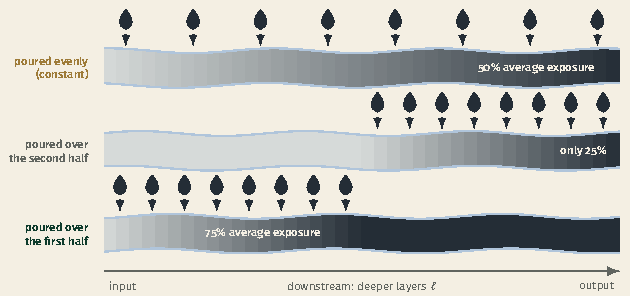
\includegraphics[width=0.93\textwidth]{figures/theory/river_ink.pdf}
\caption{A set amount of ink is distributed along a river with the goal of corrupting every cross section as much as possible. Front-loading and letting the current propagate the ink forward is the way to go. The ink is carried downstream without fading, and the percentages show average exposure along the river.}
\label{fig:river_reach}
\end{figure*}

Maximizing $\xi_{\rm eff}$ is equivalent to minimizing $\xi_{\rm eff}^{-1}$, so in the continuum limit ($x=\ell/L$) we obtain the constrained variational problem
\begin{equation}
\min_{h}\int_0^1 h(x)^{1/2} dx \qquad {\rm s.t.}\qquad \int_0^1 h(x) dx=\bar h.
\end{equation}
Since $h^{1/2}$ is concave, Jensen's inequality gives the maximum at the constant schedule. The chord bound $h^{1/2}\ge h/h_{\max}^{1/2}$ gives the minimum, attained by saturating the box constraint almost everywhere. Equivalently, any schedule that takes values in \(\{0,h_{\max}\}\) with active fraction \(f=\bar h/h_{\max}\) is optimal for the mean-field functional. A front-loaded representative, selected below by regularization reach, is
\begin{equation}
h(x)= \begin{cases} h_{\max}, & 0\le x\le f,\\
0, & f<x\le 1, \end{cases} \qquad f=\frac{\bar h}{h_{\max}},
\end{equation}
where \(x=0\) denotes the input side. All permutations of this saturated set give the same $\xi_{\rm eff}$ in the surrogate; we choose an ordering using the regularization-reach heuristic below. For finitely many layers, at most one layer remains unsaturated to meet the exact budget. These conclusions apply to the leading-order objective with weak $h_{\max}$; abrupt schedules need not track their local fixed points, and the full recurrence need not be permutation invariant. For this representative, uniform dropout yields $\xi_{\rm eff}\sim \bar h^{-1/2}$ while the step schedule gives
\begin{equation}
\frac{\xi_{\rm eff,step}}{\xi_{\rm eff,uniform}} = \sqrt{\frac{h_{\max}}{\bar h}} \;\ge\; 1.
\end{equation}
For kinked activations at $t=0$, one has $\xi^{-1}\propto h^{1/3}$, so the objective becomes $\int_0^1 h(x)^{1/3}dx$, which is also concave and therefore the same conclusion immediately follows.

\paragraph{Where should the ink enter?}
Dropout is used to ``corrupt'' the network so as to prevent it from memorizing certain ``paths'' from input to output. A toy model for understanding how to best corrupt every part of the network with a set amount of damage is to imagine a similar system: a river where a set amount of ink is to be distributed with the goal of corrupting every cross section as much as possible. Reframed this way, it is obvious that front-loading and letting the current propagate the ink forward is the way to go. While this serves as an intuitive explanation, regularization reach makes this intuition explicit.

To make the toy model precise, use normalized depth $x=\ell/L$ and write $j(x)=h(x)/\bar h$ for the injection density, with $\bar h>0$ and $\int_0^1j(x)\,dx=1$. In the limit of negligible attenuation shown in Fig.~\ref{fig:river_reach}, the accumulated exposure at $x$ and its average along the river are
\begin{align}
E(x)&=\int_0^x j(s)\,ds,\\
\bar E&=\int_0^1 E(x)\,dx
       =\int_0^1(1-s)j(s)\,ds.
\end{align}
Uniform injection has $j=1$ throughout; early and late injection have $j=2$ over their respective halves. Thus
\begin{equation}
\bar E_{\rm early}=\tfrac34,\qquad
\bar E_{\rm uniform}=\tfrac12,\qquad
\bar E_{\rm late}=\tfrac14.
\end{equation}
All three schedules deliver the same total ink to the outlet, but expose different amounts of the river along the way.

\paragraph{From the river to the network.}
The river motivates choosing among the saturated profiles with equal $\xi_{\rm eff}$ by maximizing downstream exposure to the perturbation (App.~\ref{app:regularization_reach}). In a network, a mask's influence can weaken as it propagates. Apply dropout only at layer \(\ell\). For masked and clean activations \(\tilde y_k^{(\ell)}\) and \(y_k\) at a later layer \(k\), define their angular decorrelation as
\begin{equation}
\eta_k^{(\ell)}
\equiv
1-\frac{\mathbb E_p[\langle \tilde y_k^{(\ell)},y_k\rangle]}
{\sqrt{\mathbb E_p[\|\tilde y_k^{(\ell)}\|^2]\|y_k\|^2}} .
\end{equation}
Thus \(\eta_k^{(\ell)}=0\) means perfect clean--masked alignment. Immediately after the mask, \(\eta_\ell^{(\ell)}=1-\sqrt{\rho_\ell}=(1-\rho_\ell)/2+\mathcal O((1-\rho_\ell)^2)\), while \(h_\ell=a(1-\rho_\ell)+\mathcal O((1-\rho_\ell)^2)\); hence \(\eta_\ell^{(\ell)}\propto h_\ell\) to leading order. In an ordered background, linearizing the downstream Gaussian channel gives \(\eta_{\ell+r}^{(\ell)}\simeq C h_\ell e^{-r/\xi_c}\), neglecting variance transients. We use a common background $\xi_c$ when comparing mask locations; at an exactly marginal clean channel, higher-order terms instead govern algebraic relaxation.

The readout perturbation \(C h_\ell e^{-(L-\ell)/\xi_c}\) is larger for later dropout, so readout variance is not the front-loading objective. Our scheduling heuristic uses downstream exposure: how much later computation trains while seeing the mask. A mask inserted early is seen, with decaying strength, by many later blocks; a late mask has less time to decay but fewer blocks left to regularize. We therefore define \(\mathcal D_\ell\) as the cumulative downstream exposure from placing dropout at layer \(\ell\), motivating
\begin{align}
\mathcal D_\ell
&\propto h_\ell\sum_{r=1}^{L-\ell}e^{-r/\xi_c} \nonumber\\
&\approx h_\ell\xi_c\left(1-e^{-(L-\ell)/\xi_c}\right)
\equiv h_\ell w_\ell .
\label{eq:regularization_reach}
\end{align}
Under this additive exposure model, \(w_\ell=\xi_c(1-e^{-(L-\ell)/\xi_c})\) decreases with \(\ell\), so maximizing \(\sum_{\ell=1}^L h_\ell w_\ell\) subject to \(\sum_{\ell=1}^L h_\ell=L\bar h\) and \(0\le h_\ell\le h_{\max}\) is a linear program solved by filling the earliest layers first. This is a proposed proxy for regularization; the link from cumulative exposure to generalization remains an empirical question.
